%%========================================================================
%% LaTeX sjabloon voor stage/projectrapport of bachelorproef
%%  HoGent Bedrijf en Organisatie
%%========================================================================

%%========================================================================
%% Preamble
%%========================================================================

\documentclass[pdftex,a4paper,12pt,twoside]{report}

% XXX: Let op: dit sjabloon is gemaakt om dubbelzijdig af te drukken
% Voor enkelzijdig, verwijder ``twoside'' hierboven.

%%---------- Extra functionaliteit ---------------------------------------

\usepackage[utf8]{inputenc}  % Accenten gebruiken in tekst (vb. é ipv \'e)
\usepackage{amsfonts}        % AMS math packages: extra wiskundige
\usepackage{amsmath}         %   symbolen (o.a. getallen-
\usepackage{amssymb}         %   verzamelingen N, R, Z, Q, etc.)
\usepackage[dutch]{babel}    % Taalinstellingen: woordsplitsingen,
                             %  commando's voor speciale karakters
                             %  ("dutch" voor NL)
\usepackage{eurosym}         % Euro-symbool €
\usepackage{geometry}
\usepackage{graphicx}        % Invoegen van tekeningen
\usepackage[pdftex,bookmarks=true]{hyperref}
                             % PDF krijgt klikbare links & verwijzingen,
                             %  inhoudstafel
\usepackage{listings}        % Broncode mooi opmaken
\usepackage{multirow}        % Tekst over verschillende cellen in tabellen
\usepackage{rotating}        % Tabellen en figuren roteren
\usepackage{natbib}          % Betere bibliografiestijlen
\usepackage{fancyhdr}        % Pagina-opmaak met hoofd- en voettekst

\usepackage[T1]{fontenc}     % Ivm lettertypes
\usepackage{lmodern}
\usepackage{textcomp}

\usepackage{lipsum}          % Voor vultekst (lorem ipsum)

\usepackage{wrapfig}
\usepackage{float}

%%---------- Layout ------------------------------------------------------

% hoofdingen, enz.
\pagestyle{fancy}
% enkel hoofdstuktitel in hoofding, geen sectietitel (vermijd overlap)
\renewcommand{\sectionmark}[1]{}

% lijn, wordt gebruikt in titelpagina
\newcommand{\HRule}{\rule{\linewidth}{0.5mm}}

% Leeg blad
\newcommand{\emptypage}{
\newpage
\thispagestyle{empty}
\mbox{}
\newpage
}

% Gebruik een schreefloos lettertype ipv het "oubollig" uitziende
% Computer Modern
\renewcommand{\familydefault}{\sfdefault}

% Commando voor invoegen Java-broncodebestanden (dank aan Niels Corneille)
% Gebruik: \codefragment{source/MijnKlasse.java}{Uitleg bij de code}
\newcommand{\codefragment}[2]{ \lstset{%
  language=java,
  breaklines=true,
  float=th,
  caption={#2},
  basicstyle=\scriptsize,
  frame=single,
  extendedchars=\true
}
\lstinputlisting{#1}}

%%---------- Documenteigenschappen ---------------------------------------
%% Vul dit aan met je eigen info:

% Je eigen naam
\newcommand{\student}{Ritchie Van Mele}

% De naam van je lector, begeleider, promotor
\newcommand{\promotor}{Johan Decorte}

% De naam van je co-promotor
\newcommand{\copromotor}{Krist Vanneste}

% Indien je bachelorproef in opdracht van een bedrijf of organisatie
% geschreven is, geef je hier de naam.
\newcommand{\instelling}{Hogeschool Gent}

% De titel van het rapport/bachelorproef
\newcommand{\titel}{Wat is VOIP, hoe beveilig ik mijn netwerk hiervoor en hoe werkt het met IPV6}

% Datum van indienen
\newcommand{\datum}{29 mei 2015}

% Faculteit
\newcommand{\faculteit}{Faculteit Bedrijf en Organisatie}

% Soort rapport
\newcommand{\rapporttype}{Scriptie voorgedragen tot het bekomen van de graad van\\Bachelor in de toegepaste informatica}

% Academiejaar
\newcommand{\academiejaar}{2014-2015}

% Examenperiode
%  - 1e semester = 1e examenperiode
%  - 2e semester = 2e examenperiode
%  - tweede zit = 3e examenperiode
\newcommand{\examenperiode}{Tweede examenperiode}

%%========================================================================
%% Inhoud document
%%========================================================================

\begin{document}

%%---------- Front matter ------------------------------------------------
%% Het voorblad - Hier moet je in principe niets wijzigen.

\begin{titlepage}
  \newgeometry{top=2cm,bottom=1.5cm,left=1.5cm,right=1.5cm}
  \begin{center}

    \begingroup
    \rmfamily
    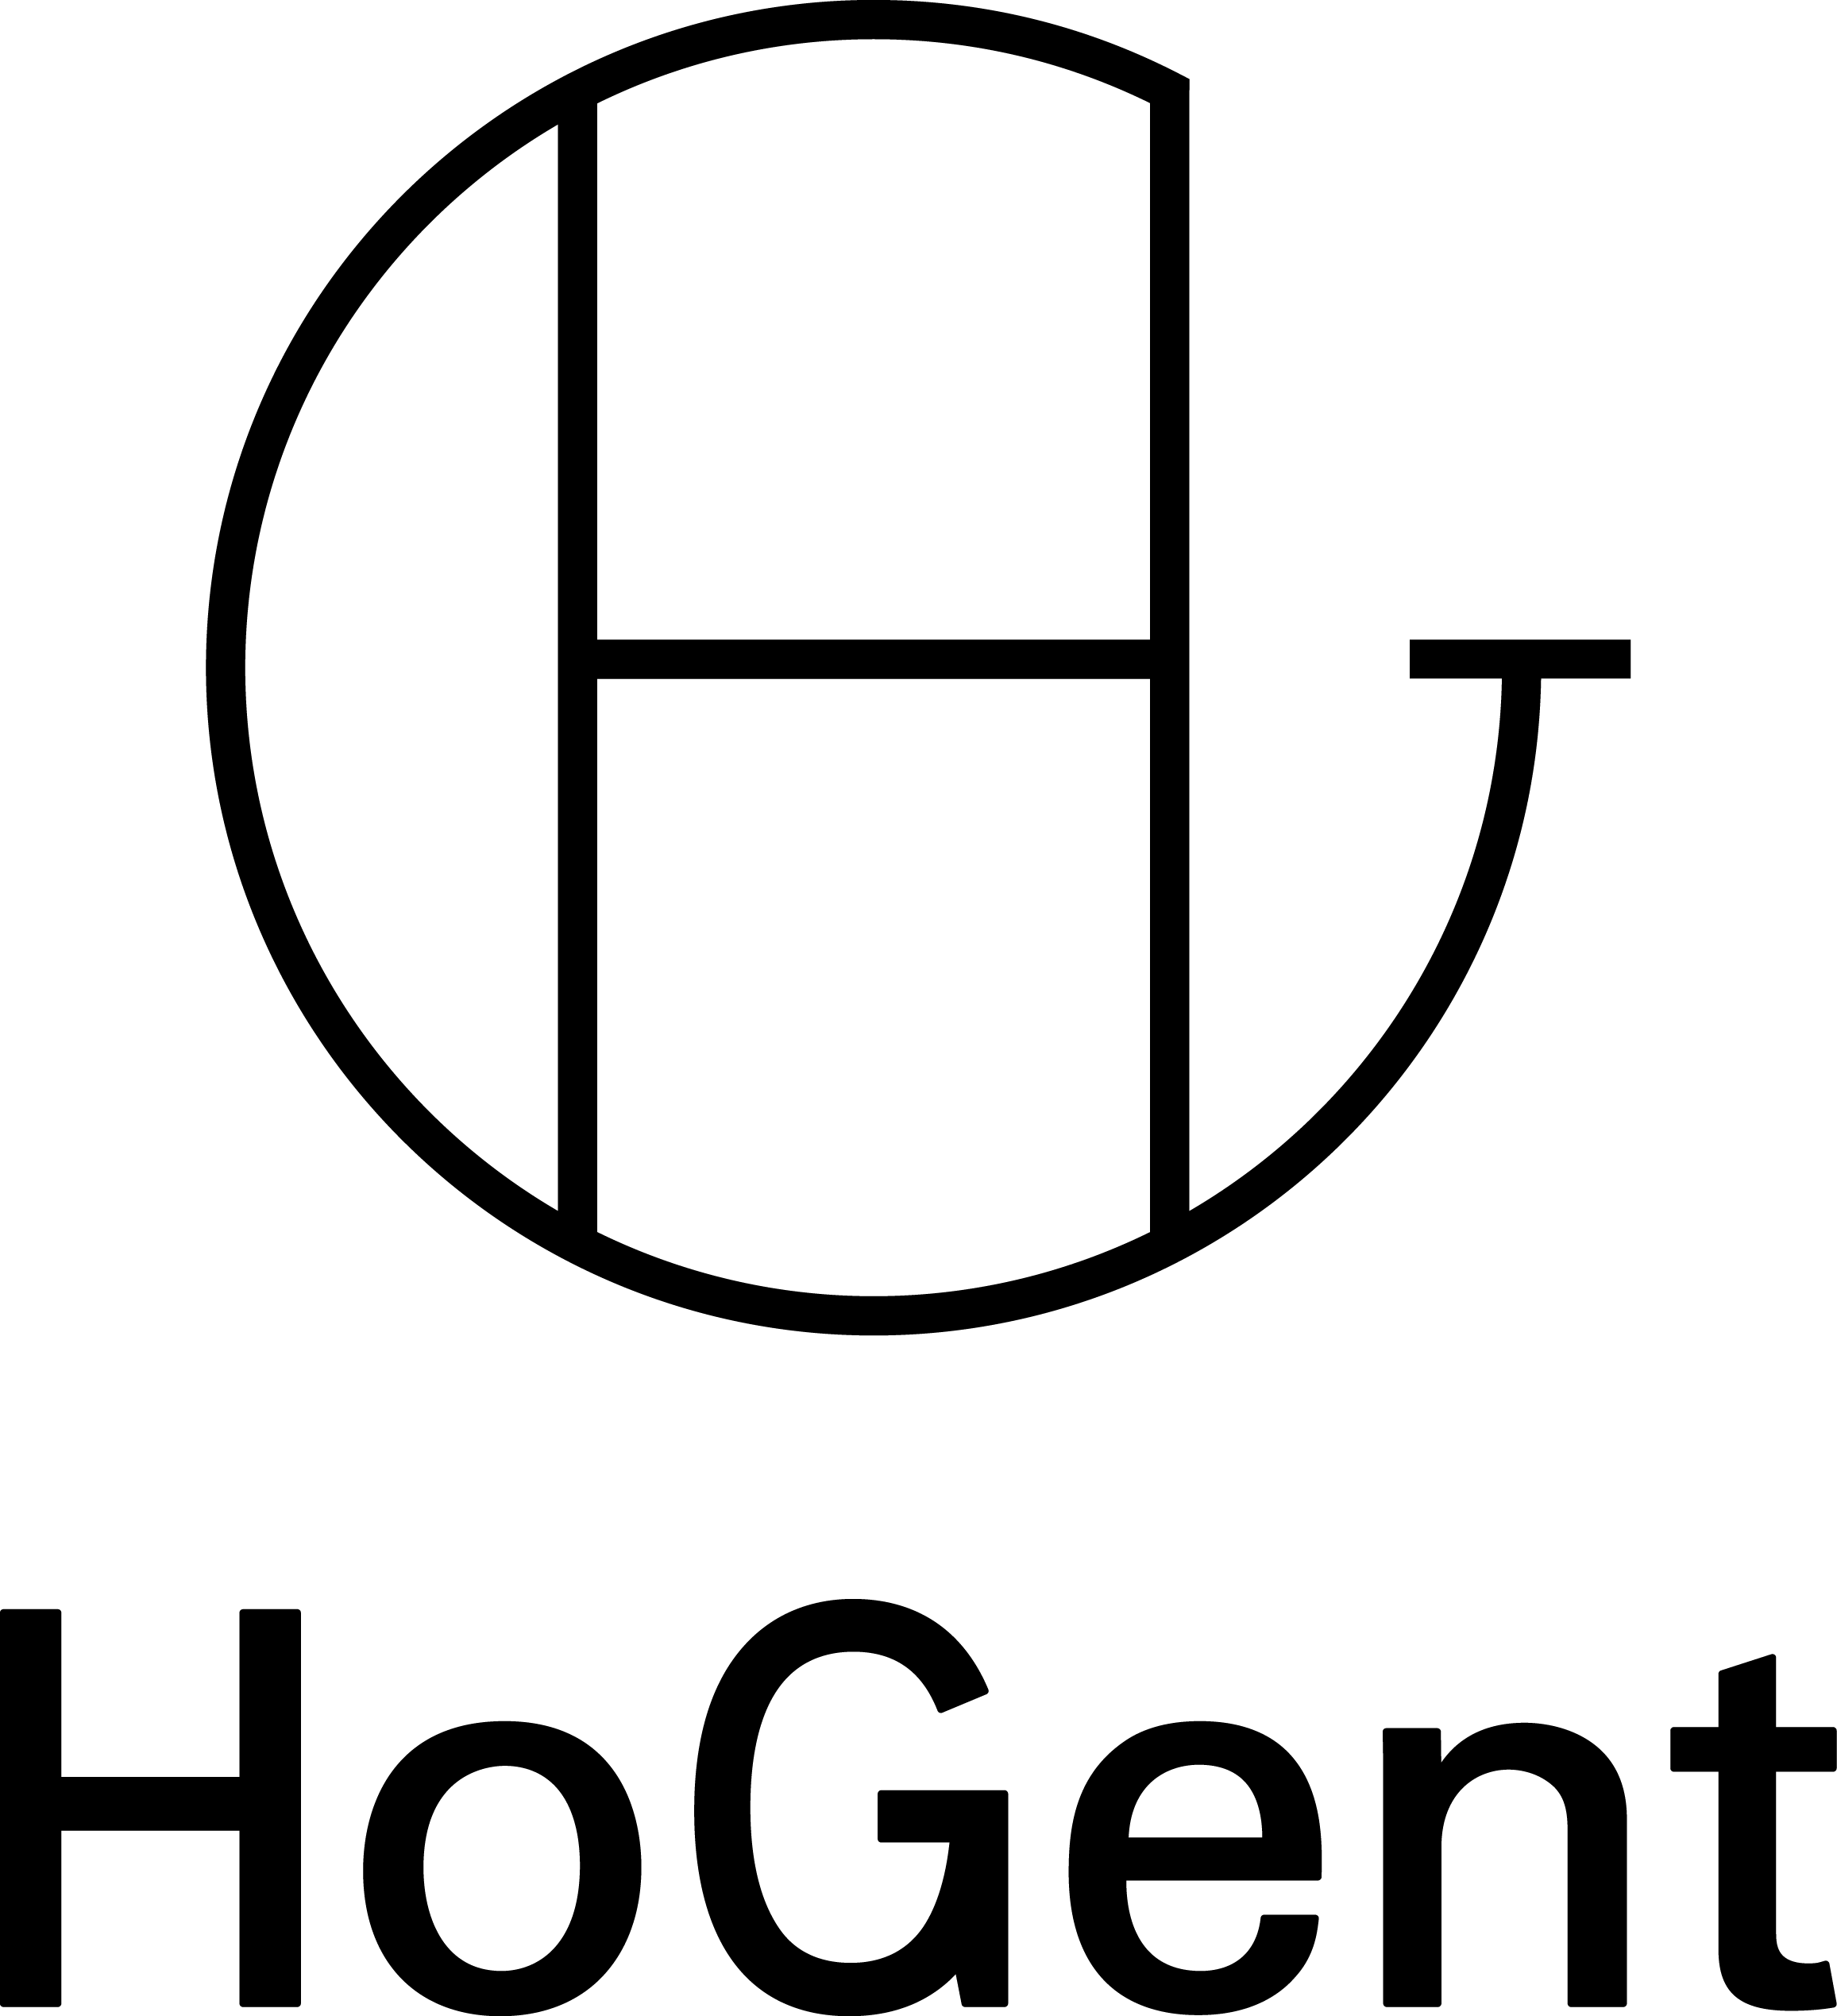
\includegraphics[width=2.5cm]{img/HG-beeldmerk-woordmerk}\\[.5cm]
    \faculteit\\[3cm]
    \titel
    \vfill
    \student\\[3.5cm]
    \rapporttype\\[2cm]
    Promotor:\\
    \promotor\\
    Co-promotor:\\
    \copromotor\\[2.5cm]
    Instelling: \instelling\\[.5cm]
    Academiejaar: \academiejaar\\[.5cm]
    \examenperiode
    \endgroup

  \end{center}
  \restoregeometry
\end{titlepage}

% Schutblad

\emptypage


\begin{titlepage}
  \newgeometry{top=5.35cm,bottom=1.5cm,left=1.5cm,right=1.5cm}
  \begin{center}

    \begingroup
    \rmfamily
    \faculteit\\[3cm]
    \titel
    \vfill
    \student\\[3.5cm]
    \rapporttype\\[2cm]
    Promotor:\\
    \promotor\\
    Co-promotor:\\
    \copromotor\\[2.5cm]
    Instelling: \instelling\\[.5cm]
    Academiejaar: \academiejaar\\[.5cm]
    \examenperiode
    \endgroup

  \end{center}
  \restoregeometry
\end{titlepage}


\begin{abstract}
% TODO: De "abstract" of samenvatting is een kernachtige (max 1 blz. voor een
% thesis) synthese van het document. In ons geval beschrijf je kort de
% probleemstelling en de context, de onderzoeksvragen, de aanpak en de
% resultaten.

Deze bachlorproef draait rond voice over IP(VOIP). In deze proef stel ik mezelf vragen en tracht daarop antwoorden te vinden. Ik ga trachten duidelijk te maken wat VOIP is en hoe ze verschilt van traditionele telefonie. Bij VOIP wordt de telefonie over een netwerk gestuurd. Ik ga dan ook onderzoeken welke invloed VOIP heeft op dit netwerk en of dit een probleem geeft voor je beveiliging. Beveiliging zowel t.o.v. het bestaande netwerk maar ook ten opzichte van je telefonie. Dan ga ik ook kijken naar op welke manieren je een onbeveiligd VOIP netwerk kan misbruiken en hoe je te beschermen tegen deze praktijken. De bedoeling is dat je na het lezen van deze proef weet wat VOIP is met alle voor en nadelen. Hoe het veilig en onveilig is en hoe je te beschermen tegen inbreuken. Deze proef sluit aan bij mijn stage bij SmartTelecom NV. Hier implementeer en beheer VOIP in nieuwe en bestaande netwerken bij klanten. Op deze manier kom ik dagelijks in contact met de voor en nadelen van VOIP. Alsook met de gevaren ervan en hoe te beveiligen tegen deze gevaren. Research via deze stage is dan ook mijn voornaamste aanpak van de probleemstelling.
 
\end{abstract}

\chapter*{Voorwoord}
\label{ch:voorwoord}
Deze thesis is in het kader van mijn bachlorproef voor toegepaste informatica aan de hogeschool Gent.\\
Het onderwerp hep ik gekozen omdat het aanleunde bij mijn stage en aangezien het een technologie is die velen kennen maar niet zozeer begrijpen of vertrouwen. 
Ik wil mijn stagementor en copromotor Krist Vanneste van SmartTelecom NV bedanken voor de hulp en research mogelijk door hem. Door heb was ik in staat om de beveiliging van een ingewikkeld netwerk te kunnen implementeren. Dit zowel voor normaal dataverkeer als voor VOIP verkeer. Uiteindelijk is mijn onderwerk geinspireerd door deze kans van samenwerking.\\
Ook bedank ik mijn stage partner Dries Vandooren voor de nuttige invloed tijdens de stage en in het onderwerp VOIP.

% TODO: Vergeet ook niet te bedankten wie je geholpen/gesteund/... heeft

\tableofcontents

% Als je een lijst van afkortingen of termen wil toevoegen, dan hoort die
% hier thuis. Gebruik bijvoorbeeld de ``glossaries'' package.

%%---------- Kern --------------------------------------------------------

\chapter{Inleiding}
\label{ch:inleiding}

Wat is VOIP? VOIP of Voice Over IP(Internet Protocol) is de technologie waar je telefonie en multimedia sessies(conference call met beeld) gaat sturen over een IP netwerk. Men verwijst vaak naar VOIP als internet telefonie. Hierbij ga je je communicatie(stem, sms, fax, … ) sturen over het internet in tegenstelling tot bij traditionele telefonie waarbij dit via een public telefonie netwerk gebeurde. In tegenstelling tot wat de naam zegt is internet verbinding niet altijd nodig bij VOIP. VOIP betekend eenvoudig dat je je communicatie gaat versturen via dezelfde protocollen als degene het internet gebruikt. Zo kan je binnen een groot bedrijf elke werknemer voorzien van VOIP telefoons en deze kunnen elkaar bellen via VOIP zonder dat ze verbinding maken met het internet. Eens ze willen bellen naar locaties buiten hun netwerk dan komt er uiteraard internet aan te pas.\\ \\
Maar we lopen vooruit op de feiten. We starten met telefonie waar het allemaal bij startte. De eerste telefoons. De eerste telefoonlijn was een directe lijn tussen 2 toestellen. Eens er meer en meer toestellen kwamen maakte men gebruik van POTS wat staat voor “Plain Old Telephone Service”. Vertaalt is dit “de eenvoudig oude telefoon service”. POTS ging over een netwerk genaamd PSTN(“public switched telephone network” of ” publiek verdeeld telefoon netwerk”). Bij directe verbindingen tussen toestellen was er sprake van een analoog signaal tussen de 2. De stem werd op deze manier overgebracht. POTS en PSTN werden mogelijk toen de ontdekking werd gemaakt dat men dit analoog signaal kon omvormen naar een digitaal signaal. Een stem die in origine analoog was kon worden omgevormd naar een digitaal signaal en kon worden verstuurd als nullen en eentjes. Een betere technologie was ontwikkeld en de basis voor wat later zou uitgroeien tot VOIP was gelegd. \\ \\
Tot op dat moment werd er gekozen om de telefonie gescheiden te houden van het opkomende computernetwerk. In computernetwerken werd er gewerkt met pakketten. Om VOIP gebruik te laten maken van deze netwerkten zou het ook zo gaan werken. VOIP gaat de geluidssignalen opsplitsen in pakketten en deze versturen over het netwerk. Deze pakketten bevatten behalve het geluid signaal ook het netwerk adres van de beller en ontvanger. En door het gebruik van pakketten werd het mogelijk om meer informatie mee te sturen om de communicatie te ondersteunen en verbeteren. \\ \\
Waar POTS specifieke benodigdheden had is VOIP enorm veelzijdig. Het werkt op verscheidene soorten netwerken. En het werkt niet alleen met VOIP telefoons maar ook met computers, Pda’s en zelf smartphones. Deze toestellen bevatten allemaal een NIC( Network Interface Card) net zoals een computer. Via deze NIC’s krijgen de toestellen dan een netwerk adres(IP-adres). Op deze manier zijn VOIP toestellen deel van je computer netwerk. \\ \\
Wat zijn nu de voor en nadelen van POTS en VOIP.\\

POTS: 
\begin{itemize}
	\item voordelen
	\begin{itemize}
		\item Het is in vele gevallen al aanwezig.
	\end{itemize}
	\item nadelen
	\begin{itemize}
		\item Het aantal main telefoonlijnen is het aantal oproepen je bedrijf tegelijk aankan. 
		\item Het aantal extenties je kan hebben is bepaald door je PBX( private branch exchange)
		\item Het werkt enkel met analoge telefoons. Geen pc's, smartphones, \ldots
	\end{itemize}
\end{itemize} 
VOIP: 
\begin{itemize}
	\item voordelen
	\begin{itemize}
		\item Ongelimiteerd aantal oproepen dat je tegelijk kan afhandelen(als je internet snel genoeg is)
		\item Ongelimiteerd aantal extenties.
		\item Bied meer aan dan enkel telefonie zoals Video calls,bellen vanop PC's, \ldots
		\item Geen gescheiden netwerk voor telefonie(geen dubbele bekabeling)
	\end{itemize}
	\item nadelen
	\begin{itemize}
		\item Er is een investeringskost bij aankoop van toestellen en PBX
	\end{itemize}
\end{itemize} 

Het is dus zeer duidelijk dat de overstap maken naar VOIP een zeer goede stap is voor bedrijven. Het geeft hen meer opties en de voordelen wegen meer door dan de nadelen. \\
Eens een bedrijf de stap maakt naar een Voice over Internet Protocol systeem is er nog een beslissing die te nemen is. Kies je voor een hosted Voip of voor een niet hosted voip.
In de voorgaande analyse ging ik er van uit dat alle apparatuur zich on site bevond. Dit wil zeggen dat alle apparatuur zoals telefoons en PBX zich op de locatie van het bedrijf bevinden.
Dit is niet de eenige mogelijkheid. Je kan er ook voor kiezen om je PBX te laten hosten door een hosting bedrijf. Hierbij zullen je VOIP telefoons geen verbinding maken met een PBX binnen je netwerk.
Maar met een PBX centrale die zich op het internet bij een bedrijf die de diensten van hun PBX aanbied. Op deze manier kan je als bedrijf kosten sparen door de aankoop van een eigen PBX systeem te vervangen door een maandelijkse hosting kost.
De voordelen van een hosted VOIP zijn dat je geen grote aankoopkost hebt, alsook dat je geen onderhoudskosten hebt. Ook kan je hierbij je VOIP telefoon toestellen plaatsen waar je wil. Je kan je toestel na het werk meenemen naar huis en daar berijkbaar zijn op het nummer van op werk.
Bij een beheren van je eigen PBX is er een investering in materiaal, maar dit geeft je de mogelijkheid je VOIP netwerk te beheren zoals jij dat wil. In theorie zou je verbindingen kunnen open stellen waarbij je je toestel ook zou kunnen thuis zetten. Dit wordt wel afgeraden omdat dit je netwerk midner veilig maakt. Meer informatie later in deze thesis.
\\
Als we naar al deze voor en nadelen kijken en we zien alle extra's dat VOIP aanbied, dan is alles positief. Nu is de vraag of en hoe VOIP dit allemaal kan. Om te begrijpen hoe VOIP werkt gaan we kijken naar een model dat al lang word gebruikt op het internet namelijk het TCP/IP model. Het TCP/IP model is een aangepaste variant van het OSI model.
TCP/IP is een groep van netwerk protocollen. En een protocol is een regel die bepaald verkeer over een netwerk gaat regelen. Je hebt protocollen voor gewoon dataverkeer en je hebt er die strikt dienen voor VOIP. Elk van die protocollen komt overeen met een laag van het TCP/IP model. Ik ga de verschillende lagen niet beschrijven tenzij het nodig is om alles te begrijpen.
Een pakket zal van start tot einde van zijn tocht elke laag 2 maal doorlopen. Eenmaal bij het verzenden en eenmaal bij het ontvangen. Waar een normaal pakket vertrekt bij de verzendende pc en aankomt bij de ontvangende computer. Vertrekt een VOIP pakket bij de beller en komt aan bij de gebelde.
Het Pakket vertrekt bij de applicatielaag en elke laag dat het doorloopt krijgt het meer informatie en veranderd het van formaat. Eens het bij de onderste laag komt(Netwerk interface) dan wordt het verstuurd over het netwerk. Eens aangekomen bij de applicatielaag van de gebelde, wordt het omgezet naar een hoorbaar formaat.
\\
Natuurlijk zijn er verschillen tussen het normale dataverkeer en VOIP verkeer. In de bovenste laag(Applicatie laag) maakt VOIP gebruik van 3 protocollen:

\begin{itemize}
	\item NTP: Network Time protocol: Dit gaat de timing verzorgen bij het verzenden van de pakketen zodat alles gebeurd in de juiste volgorde en op die manier de kwaliteit te garanderen.
	\item RTP: Real-time Transport Protocol: Gaat end-to-end netwerk transport functionaliteiten toevoegen.
	\item RTCP: Real-time Transport Control Protocol: Dit gaat het geluids signaal controleren op aflevering en controle functies toevoegen.
\end{itemize}

Ook in de transport laag is er een verschil. Waar traditionele datapakketten gebruik maken van TCP, gaat VOIP net zoals Videoconferencing gebruik maken van UDP(user datagram protocol). TCP is een trager protocol dan UDP, dit is omdat TCP meer controleerd op ontvangst van pakketten. UDP is sneller omdat het dit niet doet. 
Als er bij normaal dataverkeer een aantal pakketten niet aankomt dan is er een probleem. Dan zijn er documenten of gegevens niet volledig. Bij VOIP mag er al eens een pakket wegvallen. Zelf al wou je het pakket opnieuw verzenden dan nog kan je dat niet. Gesproken taal is sequentieel en je kan dus een deel van het begin niet op het einde erbij plakken.
Daarom is er dus gekozen voor UDP. 



\begin{figure}[h]
\caption{Het OSI model naast het TCP/IP model.}
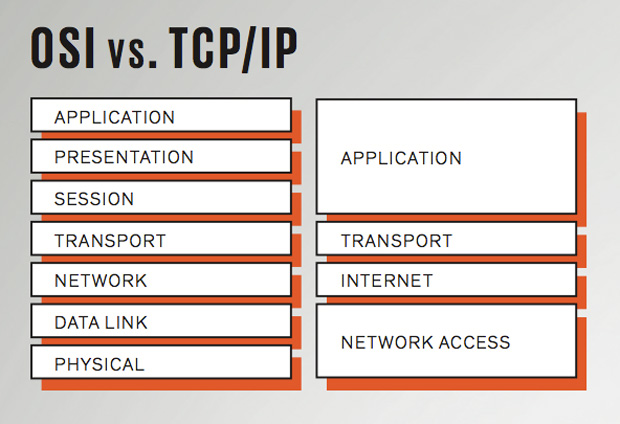
\includegraphics[scale=0.8]{img/TCP}
\end{figure}


\newpage

\section{Probleemstelling en Onderzoeksvragen}
\label{sec:onderzoeksvragen}
VOIP is een nieuwe technologie, en een nieuwe technologie toevoegen aan je netwerk levert mogelijk problemen op. 
Zoals eerder vermeld gebruikt VOIP het zelfde netwerk als je standaard netwerk data verkeer. Dit betekend dat alle beveiligingsrisico's en dreigingen dat gewoon verkeer heeft, dat deze ook dreigingen zijn voor VOIP. VOIP heeft, in tegendeel tot dataverkeer, nog geen echte standaard. Ook moet er bij VOIP rekening gehouden worden met QOS(quality of service). Een super veilig systeem met slechte kwaliteit van gesprekken is geen goed systeem. Er moet dus een middenweg gevonden worden om het systeem zo veilig mogelijk te maken zonder in te boeten aan QOS.
Nu ga ik dit alles opsplitsen in 3 categorieën.

\begin{itemize}
	\item Zijn er problemen in samenwerking met andere technologieën?
	\item Wat zijn de beveiligingsdreigingen van VOIP?
	\item Hoe werkt VOIP met IPV6?
\end{itemize}

\subsection{Samenwerking met andere Technologieën}

	\paragraph Kan VOIP ervoor zorgen dat de werking van je netwerk in het gedrang komt? Dan denk ik niet aan inbreuken via de VOIP maar eerder of de benodigdheden voor VOIP en de netwerklast die dit veroorzaakt problemen geeft voor de andere zaken die gebruik maken van het netwerk. Uiteraard is er ook de mogelijke last voor VOIP als het zich op een netwerk bevind met een reeds bestaande hoge netwerklast. Hoe zal VOIP werken in zo'n omgeving.

\subsection{Beveiligingsdreigingen}
Hier ga ik opsommen wat de voornaamste dreigingen zijn op het gebied van beveiliging van VOIP systemen. Je hebt dreigingen gericht naar het verkrijgen van informatie, het voordoen als iemand anders en het verstoren van gesprekken. 

	\paragraph Met behulp van packet sniffing software kan je de packetten van VOIP bekijken. Dit geeft je informatie over welk nummer op welk IP-address belt naar welk nummer. Deze informatie kan misbruikt worden. Door middel van bijvoorbeeld VOMIT,voice over misconfigured internet telephones, kan je de datastream van VOIP gesprekken omzetten naar een beluisterbaar formaat. 			Op deze manier kan je gesprek letterlijk worden afgeluisterd. Alle gevoelige informatie is dan dus niet meer veilig.

	\paragraph Zoals vroeger met traditionele telefonie is er bij VOIP ook altijd belang naar het verkrijgen van gratis telefonie. Men noemt dit phreaking. Hierbij gaat een fout individu trachten toegang te krijgen tot je VOIP netwerk. Op deze manier gaat deze persoon dan kunnen bellen op kosten van de eigenaar. Hij gaat dit trachten te doen door de authenticatiegegevens van een VOIP 			gebruikter te verkrijgen.

	\paragraph Indien je je netwerk veiliger maakte met de implementatie van een aparte vlan voor je VOIP telefonie is er de kans dat een individu gaat trachten toegang te krijgen tot je telefonie vlan door middel van VLAN hopping. 

	\paragraph Er zou iemand kunnen proberen om de gesprekken te verstoren. Dit is mogelijk door geluid pakketen te injecteren in de communicatie stream. Op deze manier kan de kwaliteit van een gesprek enorm verminderen, de twee sprekers kunnen zelf voor langere periodes stilte horen.

	\paragraph VOIP telefoons zijn zoals computers ook toestellen op je netwerk. Dit laat hen kwetsbaar voor een DOS aanval. Op deze manier kan iemand de telefoon spammen met onnodig veel SIP calls. Hierdoor wordt het toestel overbelast en kan het niet meer bellen of gebelt worden.

	\paragraph Waar traditionele telefoons een nummer hebben hebben VOIP telefoons een IP address. Traditionele telefoons krijgen soms reclame oproepen. Bij VOIP oproepen is het mogelijk om via scripts naar enorme hoeveelheden IP addressen reclame boodschappen te sturen. Degene toe terecht  komen bij toestellen zouden voor de zender voordelig zijn maar niet voor de eigenaar 			van dat toestel. Deze manier van reclame spamming noemt SPIT(Spamming over Internet Telephony).

 
\subsection{VOIP met IPV6}
	
	\paragraph Nu het duidelijk is dat we op het internet met een enorm tekort zitten aan publieke IP adressen is het dan ook geen verrassing dat er een nieuw internet protocol aankomt. Dit nieuwe protocol komt in de vorm van IPv6(Internet Protocol Versie 6). Elke overstap naar een nieuw protocol, van welke aard dan ook, brengt veranderingen met zich mee. Het zorgt voor vernieuwing 		maar het zorgt er ook voor dat je als gebruiker je netwerkinfrastructuur moet aanpassen zodat het met dit nieuwe protocol kan werken. \\
	Het is dan ook logisch dat we ons moeten afvragen wat de impact zal zijn van IPv6 op ons netwerk. En in het bijzonder de invloed op VOIP binnen ons netwerk? In dit deel zal ik onderzoeken wat de voordelen zijn voor VOIP en hoe we ons zullen moeten aanpassen om VOIP te laten werken met IPv6.

% TODO: Wees zo concreet mogelijk bij het formuleren van je
% onderzoeksvra(a)g(en). Een onderzoeksvraag is trouwens iets waar nog
% niemand op dit moment een antwoord heeft (voor zover je kan nagaan).

\chapter{Methodologie}
\label{ch:methodologie}

\paragraph Voor ik startte met mijn stage en mijn bachelor proef, was mijn kennis over VOIP vrij miniem. Ik wist in grote lijnen wat het deed maar niet zozeer hoe het dat deed. Mijn eerste stap naar het oplossen van mijn vragen was eenvoudig. Mijn stageliep ik aan het bedrijf SmartTelecom NV. Dit bedrijf is een provider van onder andere VOIP systemen. Door mee te lopen met mijn stagementor Krist Vanneste kreeg ik als het ware een spoedcursus over VOIP. De eerste weken leerde ik hoe VOIP werkte en waar je op moest letten. We startte bij aan de basis met telefoons en werkten stap voor stap op naar centrales en hele netwerken. Ik hielp onder andere met het implementeren van VOIP in zowel bestaande als nieuwe netwerken. Op deze manier kwam ik veel te weten over de praktijk van de zaak.een voorbeeld hiervan is dat bestaande netwerken soms niet optimaal zijn opgebouwd. Deze werken dan wel voor de basis toepassingen maar eens je er VOIP bij implementeerd zijn er problemen. 
\paragraph De tweede fase van mijn onderzoek was mijn bevindingen te gaan staven. Ik had ideeën over hoe VOIP in elkaar zit en waar je op moet letten bij het implementeren. Maar alvorens ik mijn bachelorproef kon beginnen schrijven moest ik uiteraard zorgen dat deze kennis correct was. Ik ben daarvoor aan het opzoeken geslaan. Ik ben beginnen opzoeken hoe VOIP werkt en wat experts zeggen dat de aandachtspunten zijn bij het opzetten van VOIP. Ik was dan ook zeer tevreden wanneer ik dit las en doorhad dat dit perfect aansloot met mijn eigen reeds vergaarde kennis.

\paragraph Waar ik bij het eerste en 2e deel de stage en opzoekwerk gesplitst deed deed ik bij mijn derde fase dit niet. In deze fase ging ik opzoek naar methoden om VOIP te misbruiken of om dit te dwarsbomen. Ik onderzocht hoe dit kon en hoe ik me ertegen kan beveiligen. Vervolgens ging ik dit controleren en implementeren bij een iets grotere klant. Deze klant is een bedrijvencentrum met vele verschillende partijen die toegang hebben tot het netwerk. Een zeer goede beveiliging was hier nodig en dit liet me toe om deze beveiligingen zelf te implementeren en te documenteren.
\newpage



% TODO: Hoe ben je te werk gegaan? Verdeel je onderzoek in grote fasen, en
% licht in elke fase toe welke stappen je gevolgd hebt. Verantwoord waarom je
% op deze manier te werk gegaan bent. Je moet kunnen aantonen dat je de best
% mogelijke manier toegepast hebt om een antwoord te vinden op de
% onderzoeksvraag.


\chapter{Samenwerking met andere Technologieën}
\label{ch:Samenwerking met andere Technologieën}

\paragraph In theorie zorgt VOIP voor geen problemen met andere technologieën en zaken die van het netwerk gebruik maken. In de praktijk zie je dat niet elk netwerk geschikt is om VOIP te implementeren.
Zoals vele technologieën verlangt VOIP dat het netwerk sterk en krachtig genoeg is. Op een piekmoment van telefonie, kan VOIP veel vergen van de bandwith van je netwerk. Hier wordt het dus direct duidelijk dat zwakke en zeer eenvoudige netwerken problemen kunnen hebben met de benodigdheden van VOIP. \\
Als we een netwerk gaan analyseren kijken we naar het volgende.

\begin{itemize}
	\item Latency: Dit is de tijdsvertraging die optreed tussen de verzender en ontvanger. Bij VOIP mag dit maximum 150ms zijn. Meer zou ervoor zorgen dat het gesprek wegvalt. Latency kan worden veroorzaakt door elk netwerk apparaat waar pakketten door gestuurd worden. En als een apparaat druk belast wordt dan kan dit zorgen voor vertraging.
	\item Jitter: Jitter is de variatie in Latency die kan voorkomen in een netwerk. De latency is niet constant het zelfde. Jitter is dus een soort van standaard afwijking. Bij VOIP blijft de jitter best onder 50ms. Vanaf hogere waarden is er een grote impact op de QOS.
	\item Packetloss: Soms komen bepaalde pakketten niet aan op hun bestemming. Dan spreken we van Packet Loss. Voor VOIP kan je  maximum 1\% verlies toestaan bij WAN en slechts 0.05\% bij LAN. Packet loss zorgt ondermeer voor een hogere Jitter, wat dan weer voor slechte QOS zorgt. 
\end{itemize}
Als een van deze waarden hun grens overschrijdt dan zal de kwaliteit van het gesprek enorm achteruitgaan. Er moet dus gezorgd worden dat het netwerk snel genoeg is en dat het goed is opgebouwd. Zodat het VOIP aankan. \\ \\
Vervolgens wordt duidelijk hoe VOIP andere technologieën kan tegenwerken en ongekeerd. Als je in je netwerk gebruikmaakt van zaken die zelf ook veel bandwidth gebruiken, dan kan een veeleisend VOIP met deze technologieën gaan vechten. Op deze manier leiden beide hieronder en gaan de werking van beiden achteruit. In het geval dat je netwerk problemen heeft met de hoge netwerklast door VOIP en andere zaken, dan heb je uiteraard enkele mogelijkheden. Allereerst is het aangeraden op te gaan uitzoeken wat het exact is dat deze hoge netwerklast veroorzaakt. En als het kan verholpen worden dan is het probleem opgelost. Zoniet dan moeten we een oplossing zoeken voor het probleem.  Het meest voor de hand liggende is het upgraden van je netwerkapparatuur zodat deze de last aankan. Soms is het wel eens dat de apparatuur goed is maar er gewoon een uitzonderlijke hoge netwerklast is. In dit geval kan je gaan prioriteren. Op het niveau van je router heb je te optie op QOS instellingen toe te voegen. Je kan verkeer gaan prioriteren.Je kan priotiseren op basis van de ethernetpoort, mac adress of poortnummer. De meest handige hiervan is prioritiseren op basis van de poort. Hier kan je dan eenvoudig weg het UDP verkeer voorang geven op het andere verkeer.\\
Dit is niet uiteraard niet Ideaal. Niet enkel VOIP maakt gebruik van UDP. Daarom heb je ook nog de optie op te prioriteren op basis van VLAN. Je splits het VOIP verkeer op in een apparte VLAN. En vervolgens geef je deze een hogere prioriteit dan het normale verkeer. Op deze manier zal het VOIP verkeer nooit leiden onder de hoge netwerklast opdat zijn pakketten voorang krijgen op dat van het gewone dataverkeer.



%% TODO: de structuur en titel van deze hoofdstukken hangen af van je
% eigen onderzoek. Elke fase in je onderzoek kan een eigen hoofdstuk krijgen. Kies telkens een gepaste titel. ``Corpus'' is *GEEN* gepaste titel

\chapter{Beveiligingsdreigingen en oplossingen}
\label{ch:Beveiligingsdreigingen}

\section{Packet Sniffing}

In de wereld van netwerken bestaat er een term genaamd packet sniffing. Dit betekend dat een persoon gaat trachten pakketten te bekijken die worden verstuurd over het netwerk. Als hij dit doet dan ziet hij alle pakketten en hun inhoud. Dus niet enkel die van VOIP. En als hij de pakketten ziet van VOIP dan is hij vertrokken. Packet sniffing is vandaag niet meer moeilijk. Er bestaan namelijk gratis programma’s voor. De meest bekende en gebruikte is Wireshark. Officieel is dit programma gemaakt voor netwerk beheerders om hun netwerk te kunnen analyseren en fouten te kunnen opsporen.  
\subsection{Hoe werkt het?}
Maar hoe gaat dit nu net in zijn werk. Het programma wireshark begrijpt de structuur of encapsulatie van verschillende netwerk protocollen of technologieën. Het toont de gebruiker welk pakket van welke aard is. De gebruiker kan dan kiezen welke pakketten van welke protocollen of technologieën hij of zij wil zien. Dus als hij of zij de pakketten filtert op VOIP pakketten dan krijgt hij een mooie lijst met enkel deze pakketten. Vervolgens kan hij gaan zoeken naar informatie in deze pakketten. Wireshark kan nog meer. Hij kan ook het onderscheid maken welke pakketten bij de welk horen. Op deze manier kan je een lijst genereren met gemaakte oproepen binnen je netwerk. Sterker nog het kan via VOMIT(voice over misconfigured internet telephones) deze pakketten omzetten naar een beluisterbaar formaat. Zo kan de gebruiker luisteren naar wat er is gezegd tijdens oproepen.

\newpage

\begin{figure}[H]
\caption{Voorbeeld van pakketten}
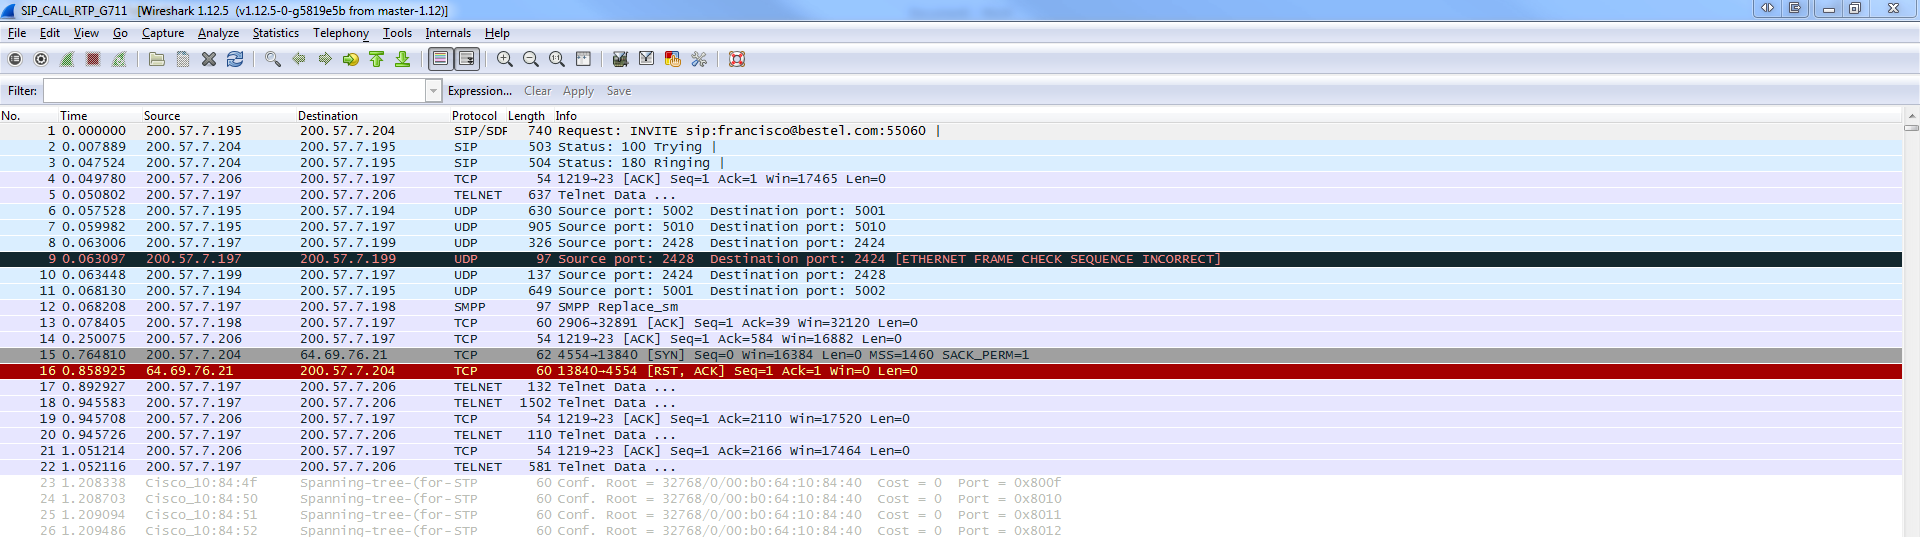
\includegraphics[scale=0.3]{img/sniffer1}
\caption{Details van een VOIP/SIP pakket}
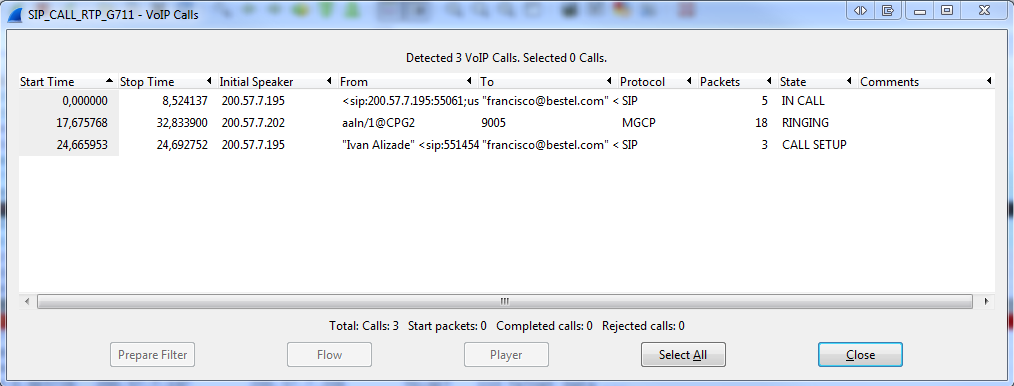
\includegraphics[scale=0.5]{img/sniffer2}
\caption{Gesprek omgezet naar beluisterbaar formaat}
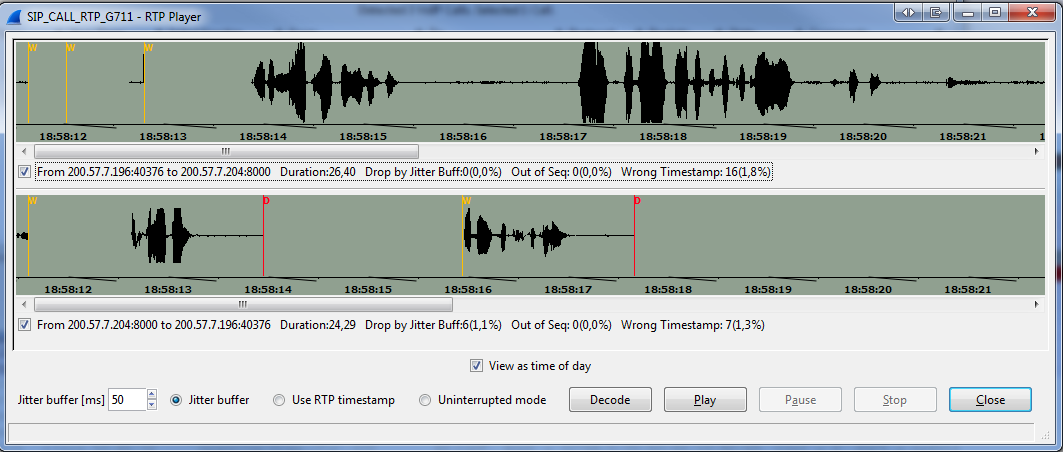
\includegraphics[scale=0.5]{img/sniffer3}
\end{figure}
\newpage

\subsection{Virtual LAN's}
Dit is een van de grootste dreigingen die mogelijk zijn voor VOIP. Elke vorm van informatie die wordt gecommuniceerd via VOIP is gewoon eenvoudig te beluisteren voor eender wie die op het zelfde netwerk zit. Het belangrijkste is vervolgens om te weten hoe we ons kunnen beschermen tegen deze packet sniffing tools. En er zijn een paar methoden die we kunnen toepassen.  \\ \\
De meest voor de hand liggende oplossing voor dit probleem is ervoor te zorgen dat het VOIP verkeer afgescheiden is van het normale netwerkverkeer. Maar een voordeel van VOIP is nu net dat het allemaal op 1 fysiek netwerk gebeurt samen met het normale dataverkeer. De oplossing hiervoor is het implementeren van VLAN's. Vlan staat voor  Virtual Local Area Network. VLAN's staan ons toe om virtueel verschillende netwerken te maken. Fysiek gebeurt alle verkeer uiteraard nog steeds over het zelfde netwerk, maar virtueel is alles gesplitst alsof ze verschillende netwerken waren. Dit geeft ons vele mogelijkheden, en ondanks dat deze proef niet over VLAN's gaat vind ik het toch nuttig om enkele van deze voordelen op te sommen aangezien VLAN's zeer handig zijn bij het beveiligen tegen verschillende dreigingen. 
\\
\\
VLAN's kunnen ingesteld worden op zowel router als switch niveau. Uiteraard heb je wel apparatuur nodig die deze technologie aankan. Zo zijn er bevoorbeeld managed en unmanaged switches. Bij een managed switch krijg je de optie om de switch te gaan instellen naargelang je netwerk setup. Een unmanaged switch is een vrij dom apparaat dat enkel de basistaken aankan.
Op het niveau van de switch kan je gaan instellen welke poorten er deel uit maken van welke VLAN. In ons netwerk zouden we alle VOIP toestellen op een VLAN stoppen en het normale verkeer op een andere. Een Vlan kan meerdere poorten bevatten en een poort kan lid zijn van meerdere VLAN's. In ons geval moeten we met dit laatste opletten. Als we een poort lid maken van zowel de normale VLAN als de VOIP VLAN, dan kan deze aan het verkeer van beide. En dit maakt het altijd minder veilig. Soms moeten we dit helaas wel doen. Bijvoorbeels als er een Computer is die VOIP software draait dan zal deze in principe ook op de VOIP VLAN moeten zitten.//
De interesante instellingen voor VLAN's gebeuren op het niveau van de router. Maar met deze interesante instellingen komt ook dat je goed moet nadenken wat je doet.  
\newpage

\begin{figure}[H]

\caption{Voorbeeld van VLAN membership in een eenvoudig netwerk \protect \footnotemark}
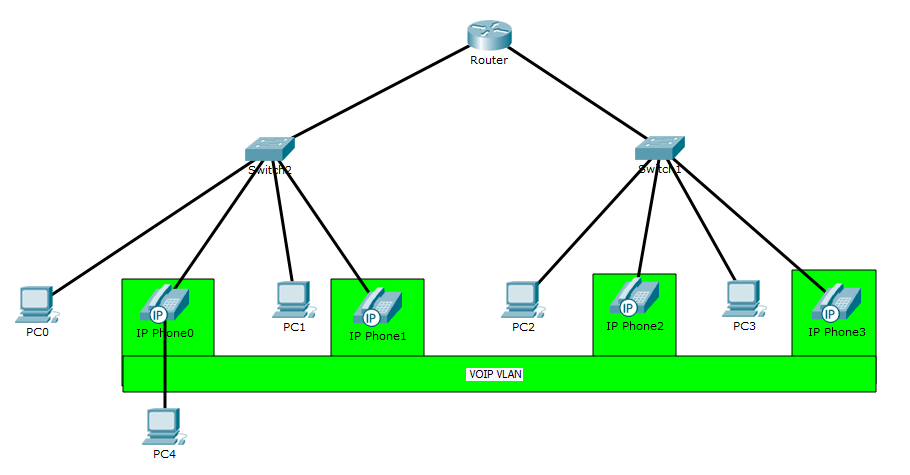
\includegraphics[scale=0.7]{img/VLAN}
\end{figure}
\footnotetext{Gemaakt met de Cisco Packet tracer Tool}

Op deze afbeelding zie je een eenvoudig netwerk met meerdere switches waar normaal verkeer en VOIP verkeer met verbonden zijn. De VOIP toestellen zijn op switch niveau toegekend aan de VLAN voor VOIP verkeer. De normale PC's zijn lid van de normale VLAN. Dit toont aan dat een gemengd netwerk nog steeds kan werken met VLAN's.
\\
\\
Nu is er nog de kans dat een persoon zich verbind met de ethernet kabel van een VOIP toestel, en op die manier toegang krijgt tot de VOIP VLAN. Hiervoor bestaat er de optie om de VLAN op een poort tagged of untagged te laten verlopen. Bij untagged wordt eender welk toestel dat verbind met die poort lid van de gespecifierde VLAN en zal zijn pakketten worden doorgestuurd naar hun bestemming. Bij tagged VLAN moeten pakketten verzonden vanaf het verbonden toestel effectief de juiste VLAN tag meekrijgen. Dus elk toestel dat gebruik moet maken van de VOIP VLAN zal dus moeten ingesteld worden alvorens deze verbinding kan maken. Als een computer dan gebruik maakt van een VOIP toestel zijn kabel, dan kan deze geen verbinding maken met het VOIP netwerk aangezien deze nooit de juiste tag heeft. \newpage
VOIP telefoons hebben vaak een interne switch. Dit laat toe dat er een ander toestel via de telefoon verbinding kan maken met het netwerk. Dit is geen probleem als we goed werken met VLAN tagging. We maken de poort lid van de VOIP VLAN maar enkel tagged. En we maken de poort ook lid van de normale VLAN maar ditmaal untagged. Op de telefoon zelf kunnen we eventueel nog instellen welke VLAN tag het 2e apparaat moet krijgen. Het toestel dat verbonden ist met de telefoon zal dan lid zijn van de normale VLAN en de telefoon van de VOIP VLAN. Zelf als de computer verbindt met de kabel bedoeld voor de telefoon, dan zal hij geen verbinding krijgen met het VLAN van VOIP. Maar wel met de normale VLAN voor het dataverkeer. 

\subsection{Encryptie}
In sommige gevallen is het afschijden van je VOIP telefonie niet geheel mogelijk. Er bestaat software \footnote{voorbeeld: http://www.xtelsio.com/} die het toestaat om te bellen met een VOIP toestel vanaf de computer. Op deze manier moet de gebruiker nooit nummer lezen van het scherm en intoetsen maar kan hij direct bellen. Dit is een zeer handige tool voor bijvoorbeeld onthaal bedienden. Om deze software te kunnen gebruiken moet deze computer toegang hebben tot het VOIP netwerk. Waar dit altijd zal zorgen voor een beveiligingsrisico is er niet direct een perfecte oplossing om deze computer tegen te houden om af te luisteren van gesprekken. \\ \\
We hebben wel een optie die het geheel veiliger maakt en het moeilijker maakt voor indiviuen om via packet sniffing kwaad te doen. We kunnen gesprekken via de telefoons versleutelen. Er bestaat een protocol genaamd SRTP(Secure Real-time Transport Protocol). Dit staat je toe om encryptie en authenticatie te implementeren op je RTP/VOIP stream. SRTP is ontwikkeld om de confidentialiteit van gesprekken en de integriteit van pakketten. Op zichzelf kan SRTP niets doen, het zorgt niet voor het versturen van pakketten. Het is enkel bedoeld om de reeds bestaande datastroom te beveiligen en te garanderen. Een VOIP gesprek bestaad uit 2 delen: de oproep(nummer draaien en verbinding maken met bestemde) en het gesprek zelf. SRTP is enkel van toepassing op het gesprek zelf. \\ \\
Maar hoe gaat het nu net in zijn werk. SRTP gaat het normale RTP pakket nemen en hieraan 2 zaken toevoegen: een Master Key Identifier en een authenticatie tag. Hieronder vind je een illustratie van het pakket. 
\newpage

\begin{figure}[H]
\caption{Voorbeeld van VLAN membership in een eenvoudig netwerk \protect \footnotemark}
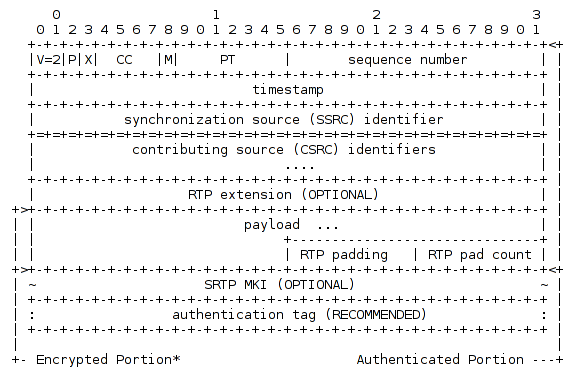
\includegraphics[scale=0.8]{img/SRTP}
\end{figure}
\footnotetext{Uit document IETF: RFC 3711 - Section 3.1}

Het genereren van deze master key gebeurt niet door SRTP. Er zijn standaarden zoals MIKEY(multimedia internet KEYing) die deze kunnen genereren. Het doel is om een master key te genereren die gedeeld is tussen 2 of meerdere gebruikers. Deze key is ook niet direct gebruikt als versleuteling maar het wordt gebruikt om een encryptiesleutel te genereren. Deze sleutel noemen we de session key. Deze session key is niet blijvend. Deze zal opnieuw gegenereerd worden. Bij het effectief versleutelen van het pakket wordt dan uiteindelijk een authentication tag gegenereerd die data over de authenticatie bevat. Deze is ook nodig bij de ontvanger om het pakket de decrypteren. \\ Voor meer informatie over SRTP verwijs ik naar het IETF document over dit protocol.\footnote{document IETF: RFC 3711}
\\ \\
Als we dit gaan samenvatten kunnen we stellen dat encryptie een zeer handige techniek is om de pakketten van VOIP gesprekken te beveiligen. In mijn mening werkt deze oplossing voor ons probleem best in samenwerking met VLAN's. Op deze manier ga je pakketten beveiligen tegen afluisteraars en ga je het aantal mogelijke afluisteraard enorm verminderen. Als we kijken naar het kost plaatje van deze oplossing dan is dit normaal nul. De enige manier om toch kosten te krijgen bij de implementatie van SRTP is als de VOIP toestellen zo verouderd zijn dat zij dit nog niet ondersteunen. Maar aangezien dit protocol al bestaat sinds 2004, zouden bijna alle toestellen van vandaag dit moeten ondersteunen.


\newpage
\subsection{Apart netwerk}
Een optie die altijd op tafel ligt is ervoor zorgen dat er helemaal geen contact is tussen je VOIP verkeer en je dataverkeer. Waar we dit virtueel doen bij VLAN(enkel intern) kunnen we dit uiteraard ook fysiek doen. Er zijn bedrijven waarbij de informatie verstuurd over het VOIP gedeelte van het netwerk enorm kritiek is. Deze bedrijven kiezen er dan ook soms voor om een apart netwerk aan te leggen enkel en alleen voor hun VOIP. Dit houd in dat het aantal netwerkapparaten bijna verdubbeld. Dit betekend ook dat ze een extra internetlijn aankopen enkel en alleen voor dit VOIP netwerk. Uiteraard is dit een zeer veilige oplossing. Er is zelf geen fysiek contact tussen het normale en het VOIP verkeer. Het is dus een eenvoudige zeer effectieve oplossing. Het heeft wel enkele grote nadelen.
\\ \\
Ten eerste is er de enorme kost die hier aan gekoppeld is. Elk stuk netwerkapparatuur moet dubbel aangekocht worden. Daarbij komt nog de maandelijkse kost voor een extra internetlijn. Nu bij kleine bedrijven is dit niet direct een probleem. Een extra router en enkele switches plus een extra internet lijn. Hier is de kost nog vrij miniem. Het probleem is dat bij bedrijven die grote gebouwen en enorm veel werknemers hebben, dat hierbij de kost enorm oploopt.\\
Een 2e netwerk betekend ook dat alles dubbel bekabeld wordt. Dit draagt niet alleen bij aan het kocht plaatje van deze onderneming, maar ook zorgt dit ervoor dat er naar elke werknemer twee keer zoveel bekabeling loopt. Opnieuw is dit niet direct een groot probleem voor kleine bedrijven, maar voor grote bedrijven wordt dit een enorme onderneming. 
\\ \\
Deze oplossing is effectief en zorgt ervoor dat er vanop het normale netwerk niet meer gezocht kan worden naar pakketten van VOIP gesprekken. Een probleem is er wel als een individue zich verbindt met de kabel bedoeld voor een VOIP toestel. Op het moment dat hij dit doet heeft hij volledige toegang tot het netwerk van VOIP. Waar we bij VLAN's een antwoord hadden hiervoor hebben we dat hier niet. 
\\ \\
Als we uiteindelijk de voor en nadelen van deze techniek op een lijstje zetten dat realiseren we ons het volgende. Deze techniek is duur en zorgt voor veel extra werk, zowel voor het aanleggen als het onderhouden van het extra netwerk. Dit extra netwerk zorgt ervoor dat er geen enkel contact mogelijk is tussen het normale dataverkeer en het VOIP verkeer. Maar voor een individue die toegang heeft tot een VOIP toestel en deze zijn kabel, is dit extra netwerk nutteloos omdat hij eenvoudig toegang kan krijgen. Deze oplossing is dus een mogelijke oplossing voor dit probleem maar niet op zichzelf. Om deze oplossing te laten werken moet er dus nog gebruik gemaakt worden van bijvoorbeeld encryptie.op deze manier kan iemand die toch toegang krijgt tot het VOIP netwerk en pakketten afluisterd, geen informatie kan halen uit deze pakketten.

\newpage
\section{Identiteits dreigingen}
Bij dreigingen voor de identiteit denk je direct aan iemand die zich voordoet als een ander op het VOIP netwerk. Zo is er bijvoorbeeld je voordoen als een ander bij het bellen, maar ook telefoons naar jou laten komen terwijl die helemaal niet voor jou bedoeld zijn. Gesprekken tussen 2 personen kan ook gecontroleerd worden door een 3e persoon die zich verborgen houd en alle gesproken informatie opslaat. Dus met dit soort dreigingen doel ik op wanneer iemand zich voordoet als iemand anders om zo aan informatie te geraken.

\subsection{Caller-ID spoofing}
Neen dit is geen proef over informatica recht, nochtans is het aannemen van een andere identiteits bij VOIP gesprekken makkelijker dan bij traditionele telefonie. In het geval van een normaal gesprek gebeurt er het volgende. Het gesprek tussen 2 toestellen verloopt via een server bij de VOIP provider of intern via de PBX centrale. In het pakket dat de gebelde ontvangt staat onder andere het server adres, de bestemmeling en de afzender. Caller-ID gaat out van wie de afzender is door wat er in dit pakket staat en dit pakket is opgebouwd door de server via wie het gesprek verloopt.\\
Stel nu dat er een slecht individu wil bellen maar de andere wil laten denken dat hij iemand anders is. Als hij toegang heeft tot de server via wie het gesprek zal gaan dan kan hij het pakket zelf opstellen en dan is het gelukt. Nu is niet niet mogelijk om de server van de provider te beïnvloeden. Er is niets wat hem tegenhoud om het gesprek via een server te laten gaan van zichzelf. Hij kan eenvoudig het pakket aanpassen zodat het een andere beller weergeeft dan zichzelf. De ontvanger zal dit pakket krijgen en bevestiging sturen naar de server van de beller. Deze server weet wie de beller is en stuurt vervolgens het pakket door naar hem. Vervolgens is het gesprek begonnen en heeft de gebelde geen idee met wie hij echt belt. In interne netwerken is er de optie om mensen zelf te laten instellen wat hun caller-ID is. Het is dan in te stellen op de centrale of deze custom caller-ID's toegelaten zijn of niet.
\\ \\
Caller-ID is niet nieuw in VOIP, het bestond al bij traditionele telefonie. Alleen is het wel makkelijker geworden bij VOIP dan vroeger. Er bestaan verschillende open source proxy server softwares zoals Asterix\footnote{http://www.asterisk.org/}. Deze zijn zeer flexibel en kunnen gebruikt worden voor vele doeleinden. Het nadeel hiervan is dan ook uiteraard dat ze bruikbaar zijn voor slechte doeleinden. 
\newpage
Je kan je niet echt beveiligen hiertegen aangezien er geen mogelijk is om te weten of de oproep komt van een correcte of incorrecte server. Het is wel zo dat bedrijven en voip providers erop worden gedrukt dat er instellingen zijn tegen caller-ID spoofing van binnenuit. Providers kunnen instellen op de centrale's(bij de bedrijven zelf) dat een oproep enkel mag verstuurd worden als de caller-ID overeenkomt met een nummer die eigendom is van het bedrijf.

\subsection{Call Hijacking}
De titel is vrij duidelijk, bij deze dreiging gaat iemand trachten een oproep niet naar de normale bestemming te laten gaan maar naar zichzelf. Op deze manier denkt de beller bij de juiste persoon te zijn terwijl dit niet zo is. Een andere vorm van hijacking is een oproep beïnvloeden dat deze via jouw beheerde proxy gaat. Op deze manier ben je een 3e partij die volledige controle heeft over de oproep. 
\\ \\
De eerste vorm van hijacking is registratie hijacking. Hierbij ga je beller doen geloven dat jij de bestemmeling bent. Elke gebruiker van het VOIP netwerk registreerd zich met de centrale met behulp van een sip account. Deze registratie gebeurt door een pakket te sturen naar de centrale met de gegevens erin. In dit pakket staat ook een tijd gedifinieerd in seconden. Dit specifieerd hoe lang de registratie geldig is. Stel dat de registratie vervalt na 3600 seconden, dan moet na een uur de registratie opnieuw gebeuren. Als op het moment dat de registratie vervalt, een aanvallend individue een zelf gemaakt registratie pakket opsteld maar met zijn IP adress in plaats van het originele. Dan denkt de centrale dat de account geregistreerd is op zijn locatie. Elke oproep die nu gemaakt wordt naar de legitime persoon komt terecht op de nieuwe locatie bij de hijacker. Deze heeft nu de mogelijkheid om zich voor te doen als de persoon die jij belt en zo mogelijk informatie te achterhalen die niet voor hem bedoeld is.\\
Deze techniek kan enkel werken als je pakketten kan afluisteren. Dus als je een of meerdere van de zaken doet uit deel 4.1, dan zou een persoon de inhoud van de pakketten niet meer kunnen bekijken. En als hij dit niet kan dan kan hij nooit het registratiepakket namaken en aanpassen.
\newpage
De tweede vorm van hijacking is uitgebreider. Hier trachten ervoor te zorgen dat een gesprek niet verloopt via de normale centrale of proxy, maar via een proxy die jezelf beheert. Om dit te berijken gaat hij beide partijen laten denken dat hij de andere persoon is, en vervolgens stuurt hij de pakketten door naar de bestemde. Zo weten de beller en ontvanger niets maar heeft hij wel volledige controle over het gesprek en de informatie die erin wordt uitgewisseld.\\
Aanschouw volgende opstelling in een voorbeeld netwerk.
\begin{figure}[H]
\caption{Voorbeeld van VLAN membership in een eenvoudig netwerk \protect \footnotemark}
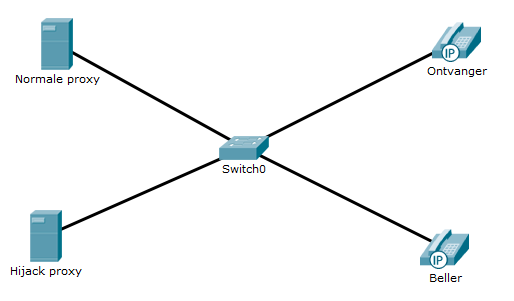
\includegraphics[scale=0.7]{img/Hijack}
\end{figure}
\footnotetext{Afbeelding gemaake met Cisco Packet Tracer}
Het volgende is het proces dat wordt doorlopen om de hijacking te voltooien.
\begin{itemize}
	\item De beller stuurt een uitnodiging om te bellen naar de ontvanger.
	\item De hijacker stuurt een antwoord bericht naar de beller zogezegt van de ontvanger. Hij geeft ook mee dat er een nieuw adres is naarwaar de oproep moet gaan.
	\item Om dit nieuw adress te bevestigen stuurt de beller een nieuwe uitnodiging naar de ontvanger maar ditmaal op het nieuwe adres, wat in feite de hijack proxy is.
	\item De hijacker stuurt een bevestigings pakket naar de beller zodat de connectie tussen hem en de beller tot stand is gebracht. 
	\item Tegelijkertijd stuurt de hijacker ook een uitnodiging naar de ontvanger met de caller-id van de beller.
	\item De ontvanger bevestigd dit in de veronderstelling dat bij met de beller in gesprek zal gaan.
	\item Tijdens het gesprek zal de hijack proxy de pakketten van de beller naar de ontvanger sturen en vice versa. 
\end{itemize}
\newpage
Vervolgens heeft de hijacker volledige controle over niet alleen het gesprek, maar ook over alle informatie die de beller en de ontvanger uitwisselen met elkaar. \\
Om dit te bekomen is het opnieuw nodig om pakketten te kunnen afluisteren. Als je dit wegneemt dan weet de hijack proxy nooit dat er een uitnodiging om te bellen is verstuurd. En dan kan hij daar ook niet op handelen.

\subsection{Besluit}
Ondanks dat er verschillende manieren zijn waarop dat je gesprek kan worden gemanipuleerd zodat je niet direct of helemaal niet naar de bestemmeling gaat, is het vrij eenvoudig om je netwerk er tegen te beveiligen. Het enige waar we ons niet tegen kunnen beveiligen is caller-ID spoofing. Uiteindelijk is de beste raad hiervoor om caller-ID niet te vertrouwen. En als er kritieke informatie zal worden gecommuniceerd zorg dan dat je weet dat je correct verbonden bent. 
\newpage

\section{Kwaliteits dreigingen}
Met dreigingen voor de kwaliteit bedoel ik de kwaliteit van de gegevens stream en van het gesprek. Doordat VOIP gebruik maakt van het netwerk, is het ook blootgesteld aan de dreigingen die een normaal dataverkeer heeft. Er zijn methoden waarop een gegevens stroom  kan worden aangevallen met als doel om verstoren te verstoren of te onderbreken. De methode waar iedereen van weet is de Denial Of Service(DOS). Ook is er DDOS\footnote{Distributed Denial Of Service: een DOS aanval op een doelwit vanop meerdere computers} maar dit heeft uiteindelijk het zelfde effect. Waar een DOS aanval op een normale dataverkeer deze kan vertragen of verstoren, is een aanval op een VOIP stream zeer snel zeer effectief. 
\\ \\
Zoals eerder al vermeld wordt een gesprek gestart met een uitnodiging\footnote{Dit is een sip pakket met de benodigde gegevens} van de beller. Als de ontvanger dit krijgt en de oproep aanvaard zal hij een bevestiging's pakket sturen naar de beller. Een persoon die een DOS aanval wil uitvoeren kan in dit geval de ontvanger bestoken met een heleboel van die uitnodiging's pakketten. Op deze manier krijgt de ontvanger zo'n grote hoeveelheid pakketten binnen dat hij deze nietmeer kan afhandelen. En de echte uitnodiging van de beller gaat dan verloren. Op deze manier kan een individue ervoor zorgen dat een persoon geen inkomende telefoons meer kan ontvangen.
\\ \\
Om dit effect te verkrijgen is er nog een andere methode. Indien de ontvanger een oproep niet aanvaard dan wordt er een annulatie pakket verstuurd. Nu kan een aanvallend individue deze annulatie pakketten versturen in naam van de ontvanger. Zo lijkt het voor de beller alsof zijn oproep niet beantwoord wordt. Waar de eerste methode in principe kan bij versleutelde pakketten kan dat hier niet. Om dit type DOS aanval te kunnen uitvoeren moet je pakketten kunnen lezen.
\\ \\
Deze 2 methoden zorgen ervoor dat een gesprek nooit tot stand komt. Nu zijn er ook mogelijkheden om een bestaand gesprek te beëindigen. Wanneer een van de 2 bellers de oproep beëindigd wordt er een vaarwel pakket gestuurd. Zo weet de andere partij dat het gesprek gedaan is. Wanneer onze aanvaller dit pakket stuurt in naam van een van de 2 bellers, dan wordt het gesprek beëindigd alsof dat de bedoeling was. Dit is opnieuw niet mogelijk als er encryptie is toegepast op het VOIP verkeer.
\\ \\
Een laatste manier om een bestaand gesprek te beëindigen is als volgt. De gegevens stroom van een voip gesprek bestaat uit RTP pakketten. Wanneer een aanvallend persoon een enorme hoeveelheid van deze pakketten stuurt naar een van de bellers, dan kan het zijn dat zijn toestel deze niet allemaal kan afhandelen. Dit zal leiden tot een slechte kwaliteit van het gesprek en uiteindelijk kan dit zelf leiden tot het beëindigen van het gesprek. Net zoals de eerste methode is deze mogelijk met of zonder encryptie. De enige maatregel die je kan nemen hiertegen is het splitsen van je normaal verkeer en je VOIP verkeer. 


\section{Voorbeeld Netwerk}

\chapter{VOIP met IPV6}
\label{ch:VOIP met IPV6}




\chapter{Conclusie}
\label{ch:conclusie}

% TODO: Trek een duidelijke conclusie, in de vorm van een antwoord op de
% onderzoeksvra(a)g(en). Reflecteer kritisch over het resultaat. Zijn er
% zaken die nog niet duidelijk zijn? Heeft het ondezoek geleid tot nieuwe
% vragen die uitnodigen tot verder onderzoek?



\bibliographystyle{apa}
\bibliography{tin-bachproef}

%%---------- Back matter -------------------------------------------------

\listoffigures
\listoftables

\end{document}
